\chapter{Blockchain: A Practical Overview and Use Cases}

\begin{quote} \emph{"The Blockchain, initially used to solve problems in
  centralized financial systems, has inherent characteristics that, depending
  on the implementation, make it suitable for a variety of use cases. This
  Chapter will provide a more in-depth exploration of the Blockchain technology
  showing some of the considerations that were taken into account, after
  analyzing the alternative implementations previously mentioned in
  Chapter~\ref{background}, to choose the Hyperledger Fabric Distributed Ledger
  Platform to achieve the purpose mentioned in Chapter~\ref{introduction}.
  Finally some pratical implementations of Blockchain based solutions created
  to solve problems in the Healthcare field or problems managing entities are
presented that provide context and show the current state of this technology in
a production environment, providing an overview of both its shortcomings and
successes thus far."} \end{quote}

\section{Trust in a Network}

Blockchain implementations are an emerging structure for distributed computing
systems that provide an accurate and unchangeable history of transactions
written to a publicly available ledger or record, even when there is no trust
relationship between the parties involved~\cite{Barclay2017}.

Banks used to keep track of their financial transactions by writing on a book
called the ledger. The ledger would be written on when a new transaction
occurred, storing all details of the transactions that occurred between the
bank and other entities. Nowadays the ledger is not a book, instead being
database storing information in a server, with the same function of recording
all the transactions that are made.

Imagine the following, Joe is on vacation and needs to borrow money from Jane,
his wife. Joe calls Jane to ask for some money and Jane tells him it will send
the money right away. Jane then proceeds to call her account manager in the
bank to transfer money to Joe. Finally Jane calls Joe to tell him the transfer
went through.  As seen on Figure~\ref{fig:centralizedvsdescentralized} Joe and
Jane need to use and trust the bank as a middle man in order to complete this
transaction. If the bank was ever to be unavailable, the database was corrupted
or if someone with  privileged access to the central database and malicious
intent was able to intercept the transactions from inside the bank then all
transactions between Joe and Jane would fail creating additional costs to all
parties involved. 

\begin{figure}[h]
  \centering
  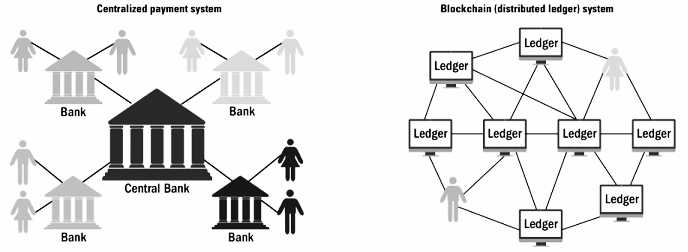
\includegraphics[width=1\linewidth]{imgs/blockchainvscentralizedNetwork.png}
  \caption{\label{fig:centralizedvsdescentralized} A comparison between a
  Centralized Banking System and a Distributed Ledger. (Source: Finance \&
  Development, 2016)}
\end{figure}

It was for a long time necessary, to establish trust between two entities, a
middle-man with a neutral stake in the transaction. While the ledger is also at
the core of the Blockchain, this technology aims to solve the dependency placed
upon third parties using decentralization and aims to make two different
entities trust each other through constant replication and through a process
called consensus.  Consensus is a mechanism that establishes a set of rules
that define if a chain of blocks is considered valid or not and depending on
the Blockchain implementation works in a different manner. With this in mind,
Blockchain implementations can be categorized into two distinct categories.

\section{Permissionless and Permissioned Blockchain Implementations}

There are three types of systems in computing, as seen on Figure
\ref{fig:typesofnetworks}. Each has their own advantages and disadvantages,
each suiting a specific use case. As previously mentioned in this Chapter,
Blockchain was created out of a desire to solve problems that are displayed in
the centralized financial systems that society is currently based upon.

\begin{figure}[h]
	\centering
	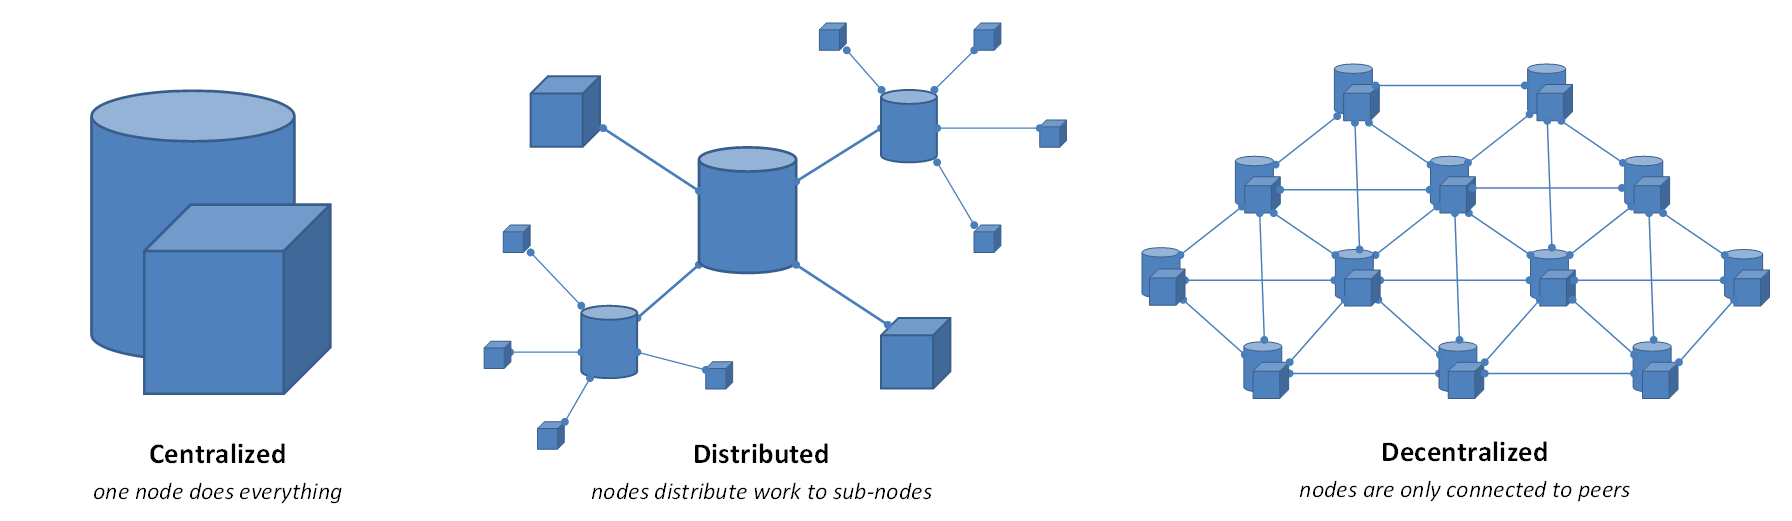
\includegraphics[width=1\linewidth]{imgs/typesofnetworks.png}
  \caption{\label{fig:typesofnetworks} A comparison between different types of
  networks. (Source: Eric Grange, 2016)}
\end{figure}

Put simply, a centralized system is one that is governed by a hierarchical
authority; examples of such being banks, credit card company’s, etc. If you
want to use a Visa card you must request access from Visa and be approved. At
any time your access to that line of credit and your funds may be made
unavailable to you and your access permanently revoked~\cite{Dreifuerst2018}.

In contrast, distributed systems are based upon the philosophy that processing
is shared across multiple nodes even if the decisions themselves may still be
centralized and use complete system state knowledge of the network. Finally, a
decentralized system is one where no single node can make a decision
individually, instead relying on the other participants to reach an agreement
and make a decision, as no single node has a complete system state knowledge.
With this in mind, a decentralized system is seen as a subset of a distributed
system.

A Blockchain is distributed by nature but internally how the system handles the
distributed nature creates two major implementation categories.

Permisionless Blockchain implementations, like the Bitcoin's and Ethereum's
Blockchain for example, have no barrier to entry. This means that anyone can,
in theory, participate in the network, write into it as a result of mining and
store data in the ledger. Permisionless implementations have some strengths;
such as being completely open, transactions are transparent while offering
anonymity or pseudo-anonymity and also take away the need for system
administrators or central servers since the network is based on peer-to-peer,
creating reduced costs to maintain and deploy \textbf{Ðapps}. On the other
hand, they are slow because every node must participate in consensus, they
operate without clear legal rules and are trust-free, meaning that no one is
really responsible if some bugs or corruption happened to cause damages to
systems based on this implementation.

Permisionless Blockchains were the first to appear and while some industries
saw benefits in using the technology, some saw drawbacks to using it in
enterprise-grade systems~\cite{Gopinath2016}.

The permissioned variant of this technology has some clear advantages for
enterprise; it is faster because consensus is done by a set of nodes instead of
the entire network, can fall on legal back on the legal system because it
features an identity service and is immediately trustworthy if the entities
that manage the network are considered themselves trustworthy because it is
auditable and there is a legal responsible entity or entities that manage the
network. However, costs when compared to the permissionless variant are higher
due to having the need for a system administrator and servers to manage the
network, feature a private membership meaning that they are closed to the
general public and managed by a set of entities and are a compromise between
the original vision of a distributed network and enterprise needs and concerns. 

Enterprises benefit greatly from the immutability of the Blockchain
architecture, in that all records cannot be changed. By adding authorised
identity services onto Blockchain, they can meet the regulatory needs of their
industries, by allowing the network to be auditable and assets to be traceable,
falling back to laws if a dispute between participating entities
occurs~\cite{Barclay2017}.

With these two variants in mind, Section~\ref{choosingHyperledger} provides an
insight into the characterists deemed important to achieve the estabilished
purposes that this project set out to achieve and explains the decision
processes behind the choice of a permissioned implementation of the Blockchain
technology being used to build a system for managing patients in Healthcare. In
Section~\ref{blockchainHealthcare} some previous Blockchain based solutions in
the Healthcare context are analyzed to take away key learnings that may be used
to improve or be aware of in designing the system.

\section{System Requirements and Starting Blocks}\label{choosingHyperledger}

After considering the project goals of investigating the suitability of a
Blockchain based system to manage patients in Healthcare, it was decided to
build a prototype of a system that would represent the network, albeit on a
smaller scale. The insights gained from developing a simple working system
would enable benefits and risks of the approach to be identified, and
opportunities for further research to be laid out.

The requirements for this project are deemed to be as follows:

\renewcommand{\labelenumi}{\Roman{enumi}.}
\begin{enumerate}
  \item The system must allow a patient to opt into the network securely.
  \item The system must allow a patient to record his medical data under the
    approval of an administrator.
  \item The system must keep information confidential, transparent and have
    high availability.
  \item The system must provide the patient with the ability to share his data
    with another entity participating in the network, for example sharing
    information with a doctor.
  \item The system must allow data  of patient to be erased in some manner if
    he wishes to do so, in order to comply with European privacy laws.
\end{enumerate}

This section  explores some Blockchain deployments and discusses the key
benefits and drawbacks of these, in regards to the suitability of usage as a
platform for developing the system.

Blockchain platforms often have different goals even tough they originate from
the realization that full centralization has major drawbacks. Ranging from open
networks, such as Ethereum which anyone can join and use, to permissioned
distributed ledgers, which can be run publicly or privately but are only open
to access and participation through a membership service, such as Hyperledger
Fabric and Hyperledger Indy.

\subsection{A Decentralized Open Platform - Ethereum}

Ethereum is a permissionless Blockchain implementation. It is a platform that
lets anyone build and use decentralized applications commonly named
\textbf{Ðapps}. It is an open-source project developed primarily by the
Ethereum Foundation and was designed to be adaptable and flexible, in contrast
to Bitcoin's Blockchain that only records financial
transactions~\cite{EthereumDocs2018}.

 It features a friendly programming language called Solidity that is influenced
 by C++, Python and Javascript that is designed to allow an easy way for
 developers to create new applications on the Ethereum platform with code of
 arbitrary algorithmic complexity in a turing complete language. Smart Contract
 application code targets the Ethereum Virtual Machine, which is then deployed
 to the Blockchain via a local Ethereum node~\cite{Wood2017,Barclay2017}.

At the heart of Ethereum is the Ethereum Virtual Machine (\textbf{evm}) as seen
on Figure~\ref{fig:evm} and, like any Blockchain, Ethereum also includes a
peer-to-peer network protocol. The Ethereum Blockchain database is maintained
and updated by many nodes connected to the network. Each and every node of the
network runs the EVM and executes the same instructions in order to maintain
consensus across the entire Blockchain. Decentralized consensus gives Ethereum
a high degree of fault tolerance, ensures zero downtime, and makes data stored
on the Blockchain forever unchangeable and
censorship-resistant~\cite{EthereumDocs2018}.

\begin{figure}[h]
	\centering
	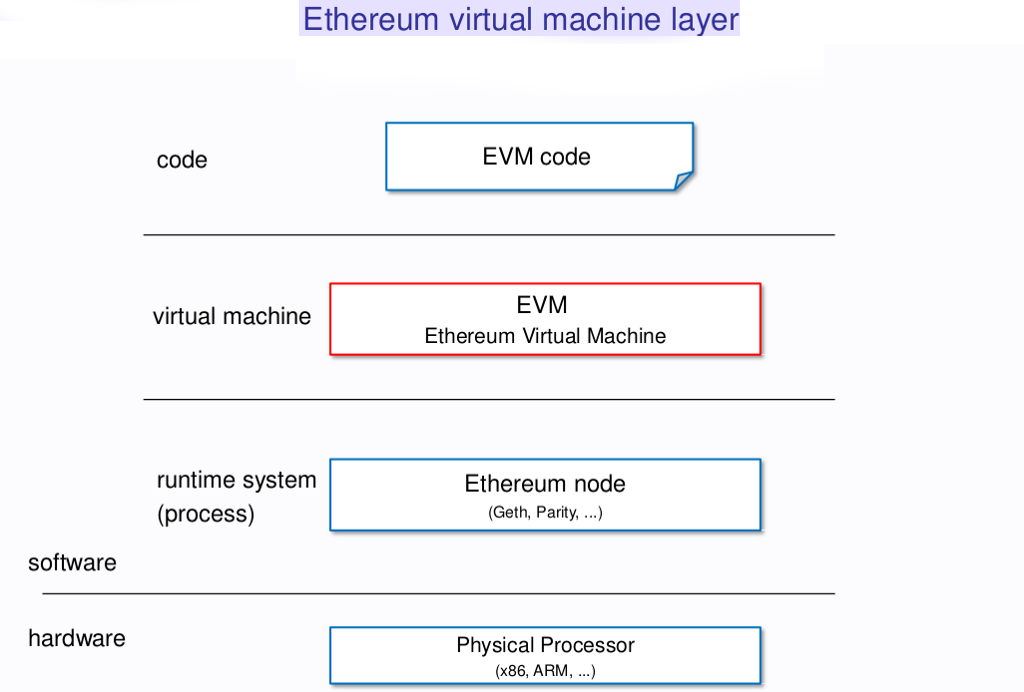
\includegraphics[width=1\linewidth]{imgs/ethereumVirtualMachine.png}
  \caption{\label{fig:evm} A diagram of where \textbf{evm} fits into the
  Ethereum Platform (Original: Vaibhav Saini, 2018)}
\end{figure}

Users must pay a small transaction fee to the network each time they execute a
transaction. This protects the Ethereum Blockchain from frivolous or malicious
computational tasks, like \textbf{ddos} attacks or infinite loops. The sender
of a transaction must pay for each step of the “program” they activated,
including computation and memory storage. These fees are paid in amounts of
Ethereum’s native value-token, ether, and then these transaction fees are
collected by the nodes that validate the network commonly called miners - which
are nodes in the network that receive, propagate, verify, and execute
transactions. Ethereum currently uses a \textbf{pow} based consensus algorithm
but plans to change to a proof of stake (\textbf{pos}) algorithm due to
environmental and financial concerns as well as reduced centralization
risks~\cite{EthereumDocs2018,EthereumPOSFAQ2018}.

Ethereum has a live production network called “mainnet” available for any
developer to deploy applications to, as well as three test networks. "Ropsten”
is based on a \textbf{pow} algorithm while "Rinkeby" and "Kovan" are based on a
Proof of Authority~\footnote{In Proof of Authority based networks, transactions
and blocks are validated by approved accounts, known as validators. Validators
run software allowing them to put transactions in blocks. The process is
automated and does not require validators to be constantly monitoring their
computers. It does, however, require maintaining the authority node
uncompromised.} (\textbf{poa}) and all of them are publicly available and free
to use~\cite{Barclay2017,EthereumTestNetworks2018}.

Ethereum has had some unforeseen problems along the way, namely the DAO heist
where a hacker took advantage of a bug in a smart contract to steal a great sum
of money. With Ethereum frequently reaching full transaction capacity, scaling
solutions are the next big investment~~\cite{ethereumScalability2018}.

There are a few proposed solutions by Buterin - sharding aims to avoid every
node processing all data in order to verify and process a transaction. When
transactions are initiated they will not be directed to all the nodes but
would instead only be directed to those depending on the shard in question.
Another solution is off chain computation where a layer apart from the
Blockchain is created and where all the computation or solving of a complex
mathematical equation takes place. This would not only take the load off the
Ethereum Blockchain but also help decrease the cost of transaction
verification and processing. This mechanism would ensure that the tasks that
account for slower transaction speeds on the Ethereum’s Blockchain do not
affect the whole network. Finally, to avoid every node having the need to
download the entirety of the Blockchain's data, the complete picture can be
stored on cloud and each node only has to store and load relevant
data~\cite{ethereumBlogScalability2018}.

\subsection{A Permissioned Distributed Ledger Platform - Hyperledger Fabric}

Hyperledger Fabric is a platform for distributed ledger solutions underpinned
by a modular architecture. It provides developers with a permissioned platform
targeted at business and enterprise that supports pluggable implementations of
different components to accommodate the complexity and intricacies that exist
across the economic ecosystem. It is an open source project initially commited
by IBM  and estabilished under the Linux Foundation, being developed by over 35
organizations and nearly 200 developers~\cite{HyperledgerFabricDocs2017}.

It supports the creation of smart contracts programs, commonly called
"chaincode" in Fabric, that are authored in general-purpose programming
languages such as Java, Go and Node.js rather than constrained domain-specific
languages (\textbf{dsl}). Chaincode runs in a secured Docker container isolated
from the peer process which consented its installation. Chaincode also
initializes and manages ledger state through transactions as well as the world
state.

At the heart of Fabric is the permissioned distributed ledger that provides a
way to secure the interactions among a group of entities that have a common
goal but which may not fully trust each other. By relying on the identities of
the participants, a permissioned ledger platform can use more traditional crash
fault tolerant (\textbf{cft}) or byzantine fault tolerant (\textbf{bft})
consensus protocols that do not require mining.

\begin{figure}[h]
  \centering
  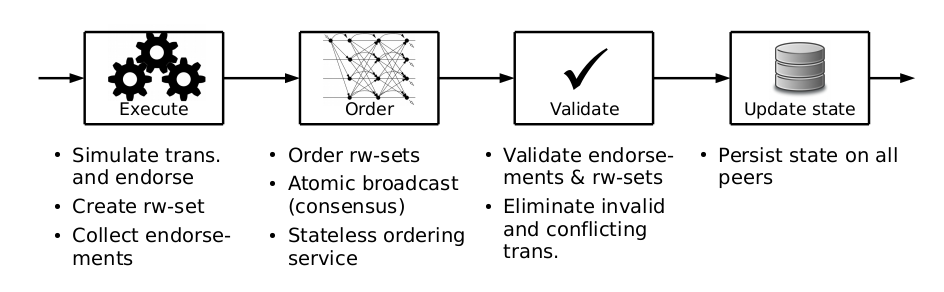
\includegraphics[width=1\linewidth]{imgs/executeOrderValidate.png}
  \caption{\label{fig:executeorder} Execute-order-validate architecture of
  Fabric (Source: IBM, 2018)}
\end{figure}

Fabric introduces the execute-order-validate Blockchain architecture as shown
on Figure~\ref{fig:executeorder} and does not follow the standard order-execute
design illustrated on Figure~\ref{fig:orderexecute} \cite{Androulaki2018}. 

\begin{figure}[h]
  \centering
  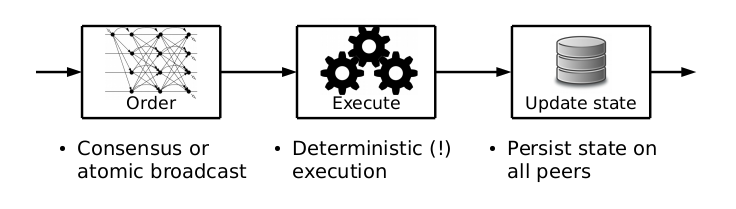
\includegraphics[width=0.8\linewidth]{imgs/orderExecuteArchitecture.png}
  \caption{\label{fig:orderexecute} Order-execute architecture in Replicated
  Services Like Ethereum (Source: IBM, 2018)}
\end{figure}

The order-execute architecture is conceptually simple, leading it to it being
currently widely implemented in replicated services like Blockchain. In this
architecture the transactions are executed sequentially on all peers  which
limits the maximum number of simultaneous transactions that can be achieved.
Additionally a Denial of Service (\textbf{dos}) attack can be mounted just by
deploying a slow performing smart contract or one with an infinite loop to the
network since the Blockchain forms a distributed computing engine.  To cope
with this issue, public programmable Blockchains with an associated
cryptocurrency, account for the execution cost of executing of the program.

Chaincode in Fabric consists of two components - the code itself, which
describes the logic of the program running in the execution phase, and the
endorsement policy that describes how a specific chaincode transaction is
validated. For example, a typical endorsement policy lets the chaincode specify
the endorsers for a transaction in the form of a set of peers that are
necessary for endorsement and subsequent successful
validation~\cite{Androulaki2018}.

In Fabric all nodes that participate in the network have an identity, as
provided by a modular membership service provider (\textbf{msp}).  A
\textbf{msp} is a component that aims to offer the abstraction of a membership
operation architecture.  It maintains the identities of all nodes in the system
and is responsible for issuing credentials that are used for node
authentication and authorization. An \textbf{msp} may define their own notion
of identity, and the rules by which those identities are governed (identity
validation) and authenticated (signature generation and
verification)~\cite{HyperledgerFabricDocs2017}.

Nodes in a Fabric network take up one of three roles:

\begin{itemize}
  \item Clients submit transaction proposals for execution, help orchestrate
    the execution phase, and, finally, broadcast transactions for ordering.

  \item Peers execute transaction proposals and validate transactions.  All
    peers maintain the blockchain ledger, an append-only data structure
    recording all transactions in the form of a hash chain, as well as the
    state, a succinct representation of the latest ledger state. Not all peers
    execute all transactions.

  \item Ordering Service Nodes (\textbf{osn}) or orderers are the nodes that
    collectively form the ordering service. In short, the ordering service
    establishes the total order of all transactions in Fabric, where each
    transaction contains state updates and dependencies computed during the
    execution phase, along with cryptographic signatures of the endorsing
    peers.  Orderers are entirely unaware of the application state, and do not
    participate in the execution nor in the validation of transactions. This
    design choice renders consensus in Fabric as modular as possible and
    simplifies replacement of consensus protocols in Fabric. 
\end{itemize}

Looking ahead, Hyperledger Fabric will continue to focus on privacy and
confidentiality with v1.2 being recently released, v1.3 and 1.4 expected to be
out this year with further emphasis on these aspects in a quarterly
cadence~\cite{hyperledgerRoadmap2018}.

\section{Choosing a Platform}
% Talk about Ethereum vs Fabric vs Indy
%TODO
